\documentclass[a4paper]{article}
\usepackage{preamble}

% Setup title
\title{PHYSICS 2 - TERM 2}
\author{Marc Sanchis}
\date{April 2024 - June 2024}

\begin{document}

% Title
\newgeometry{top=2cm, bottom=5.5cm}
\maketitle

% Table of Contents
\renewcommand{\contentsname}{}
\tableofcontents

% Body
\newpage
\restoregeometry
\pagestyle{fancy}
\setcounter{section}{4}

\section{Magnetism in Matter}

\subsection{Magnetic Behaviour}
Materials fall into three groups based on their magnetic behaviour:

\begin{itemize}
    \item \textbf{Diamagnetic}: It has a weak, opposite-direction reaction to a $B$ field.
    \item \textbf{Paramagnetic}: With no $B$ their electrons have a defined magnetic moment, and when a magnetic field is applied, they have a slight attraction towards it.
    \item \textbf{Ferromagnetic}: Same as Paramagnetic, but its dipoles are aligned even before the $B$ the field is applied and has a very strong, attractive reaction.
\end{itemize}

For $B_{0}=0$, the vacuum has $(\vec{m}=\vec{0}, \vec{B}=\vec{0})$, Diamagnetic $(\vec{m}_{atomic}=\vec{0}, \vec{m}=\vec{0},\vec{B}=\vec{0})$, Paramagnetic $(\vec{m}_{atomic}\neq \vec{0},\vec{m}=\vec{0}\vec{B}=\vec{0})$, Ferromagnetic $(\vec{m}_{atomic}\neq\vec{0},\vec{m}\neq\vec{0}),\hspace{1ex}\vec{0}\in D:\sum\vec{m}$ .

For $B_{0}\neq 0$, the vacuum has $\vec{B}_{total}=\vec{B}_{0}$, Diamagnetic $\vec{B}_{total}<\vec{B}_{0}$, Paramagnetic $\vec{B}_{total}>\vec{B}_{0}$, Ferromagnetic $\vec{B}_{total}\gg \vec{B}_{0}$ .

\begin{align}
\vec{M}=\frac{d\vec{m}}{dv},\hspace{4ex}J_{S}&=|\vec{M}|,\hspace{4ex}dm=dI\cdot dS \\
\vec{B}_{total}&=\vec{B}_{0}+\vec{B}_{JS}
\end{align}

\note{If the magnetisation $M$ is constant, amperian bound currents appear in the material surface}
\begin{figure}[h]
    \centering
    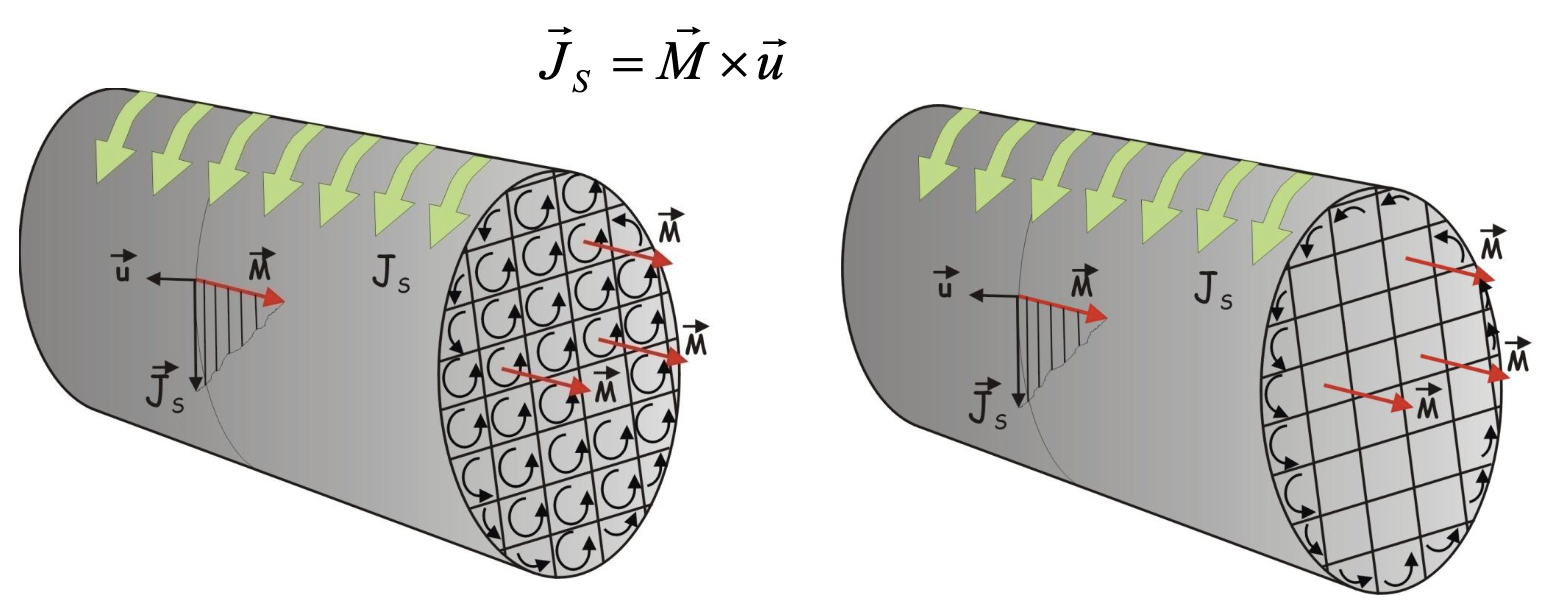
\includegraphics[width=0.5\textwidth]{IMG/js.png}
    \caption{Amperian bound currents appearing}
    \label{fig:js}
\end{figure}

\subsection{Magnetic Excitation}
\subsubsection{The H field}
The $H$ field only depends on the free current.
$$
\vec{H}=\frac{\vec{B}}{\mu_{0}}-\vec{M}, \hspace{4ex}\vec{B}=\mu_{0}(\vec{H}+\vec{M})\to B^*=\mu_{0} (H+M)
$$
$H$ can be demonstrated in two equivalent ways:
$$
\begin{cases}
&\oint \vec{H}\cdot d\vec{l}=\int_{C} \frac{\vec{B}}{\mu_{0}} \, d\vec{l}\,-\int_{C}^{} \vec{M} \, d\vec{l}\, = \frac{1}{\mu_{0}}[\mu_{0}nlI+\mu_{0}J_{S}l]-J_{S}l=nlI \\
&\oint_{C} \vec{H}\cdot d\vec{l}=Hl
\end{cases} \hspace{1ex}\to \boxed{H=nI}
$$
and
$$
\to\begin{cases}
B=\mu_{0}[nI+J_{S}]=\mu_{0}[nI+M] \\
B^*=\mu_{0}(H+M)
\end{cases}\hspace{1ex}\to \boxed{H=nI}
$$

\subsubsection{Ampère's Theorem for H}
Per Ampère's theorem for $H$:
$$
\oint_{C}\vec{H}\cdot d\vec{l}=I_{f r e e}, \hspace{4ex}Curl(\vec{H})=\vec{J}_{f r e e}
$$

\subsubsection{M-H Relationship}
The relationship between $M$ and $H$ is
$$
\vec{M}=\chi \vec{H}
$$
For diamagnetic materials $0<\chi\ll-1$, paramagnetic $0>\chi\ll 1$, ferromagnetic $1000<\chi<8000$.

$$
\vec{H}=\frac{\vec{B}}{\mu_{0}}-\vec{M}=\frac{\vec{B}}{\mu_{0}}-\chi \vec{H} \to \vec{B}=\mu_{0}(1+\chi)\vec{H}=\mu \vec{H}
$$
$$
\mu_{r}=\frac{\mu}{\mu_{0}}=1+\chi
$$

\end{document}
